\Chapter{Tervezés}

\Section{Koncepció}
Mint látni lehet a Multi2Sim-nél, a szimuláció lehetséges megoldása a problémának, viszont roppant bonyolult és erőforrásigényes. Ebben a dolgozatban megpróbálunk egy sokkal egyszerűbb, kevésbé pontos megoldást kínálni ami remélhetőleg sokkal szemléltetőbb. 

Mivel a hardveres futás szimuláció kicsit bonyolult, ezért azt elvetve marad a futó program elemzése. Erre lehetőséget biztosít a GDB, egy GNU project debugger, de ennek a precizitása kétséges, illetve csak a házigazda program futásának elemzésére alkalmas. A másik vizsgálandó megoldás a forráskód elemzése.

 Az OpenCl működésének ismeretével lehetséges lehet olyan alkalmazást létrehozni, ami a forráskódban felismeri az OpenCL elemeit, és helyesen megtippeli hogy azok mit csinálnának. Így felépíthető lenne egy modell az adott OpenCL program működéséről amit már csak megjeleníteni szükséges.
 
\Section{Triviális elemek}
Az OpenCL programok egy jelenntős része a házigazda programban történik, aminek nagyon sok kötelező eleme van, mint például a platformok keresése. Feltételezhetjük, hogy ezek a triviális elemek az analizálandó programban is megtalálhatóak, tehát nincs szükség feleslegesen erőforrásokat pazarolni a megkeresésükre. Viszont néhánynál szükség lehet megnézni, hogy milyen argumentumaik vannak, illetve hány darab van belőlük. Ekkor a házigazda program nagy része már modellezve is van.

Triviális elemeknek tekinthetők a platform, memóriák felszabadítása, kernel létrehozás, OpenCL program készítése, parancs sor készítése, környezet létrehozása, egyebek.



\Section{Teendők a kernellel}
Igazából a kernelben található konkrét műveletek elemzési, vizualizációs szempontokból elhanyagolhatók. Ami ott fontos és ajánlott vele foglalkozni, azok a szinkronizációs függvények, például egy sorompót érdemes lehet grafikusan megjeleníteni.

\Section{Munka elemek}
Egy fontosabb részlete az elemzésnek a munka elemek számának megállapítása. Ideális esetben megvan határozva a munkacsoport elemeinek száma, és ez kiolvasható a forráskódból. Ha ez nincs meghatározva, meg kell tippelnünk a számukat az OpenCL specifikáció alapján. Ezután rá tudunk jönni a munkacsoportok számára az NDRange és a kernel input alapján.

\Section{Program felépítése}

\begin{figure}[h]
\centering
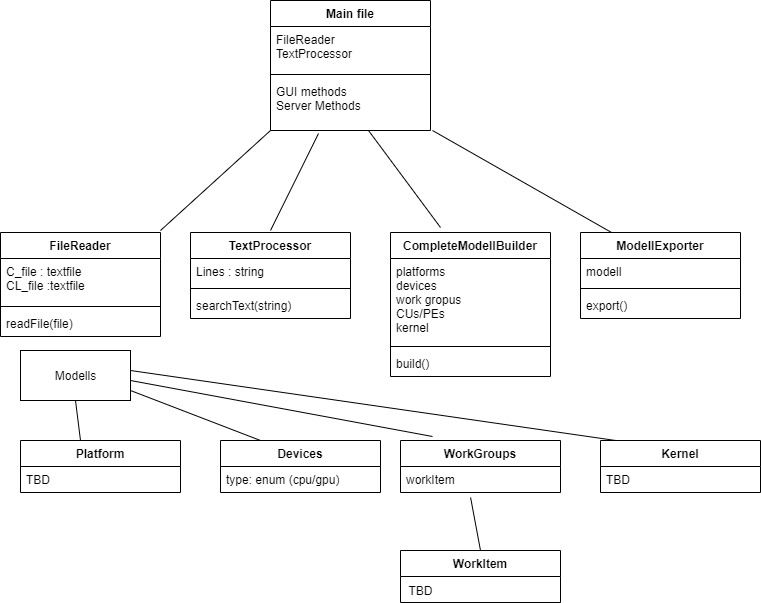
\includegraphics[scale=0.5]{images/UML.jpg}
\caption{INITIAL UML osztálydiagram}
\label{fig:uml}
\end{figure}

A program működése a következő:

Beolvassuk a forrásokat, lehetőleg valamilyen grafikus felületen át, majd feldolgozzuk először a házigazda forrásfájlt. Megkeressük benne az OpenCl függvényeket, és szükségszerűen modelleket rendelünk melléjük, például a \texttt{clCreateKernel} metódust észlelve létrehozunk egy Kernel objektumot. Ha ezzel készen vagyunk összeállítjuk őket egy teljes modellé, amit exportálunk a frontend felé.

\Section{Táblázatok}

Táblázatokhoz a \texttt{table} környezetet ajánlott használni.
Erre egy minta \aref{tab:minta}. táblázat.
A hivatkozáshoz az egyedi \texttt{label} értéke konvenció szerint \texttt{tab:} prefixszel kezdődik.

\begin{table}[h]
\centering
\caption{Minta táblázat. A táblázat felirata a táblázat felett kell legyen!}
\label{tab:minta}
\begin{tabular}{l|c|c|}
a & b & c \\
\hline
1 & 2 & 3 \\
4 & 5 & 6 \\
\hline
\end{tabular}
\end{table}

\Section{Ábrák}

Ábrákat a \texttt{figure} környezettel lehet használni.
A használatára egy példa \aref{fig:cimer}. ábrán látható.
Az \texttt{includegraphics} parancsba 
Az ábrák felirata az ábra alatt kell legyen.
Az ábrák hivatkozásához használt nevet konvenció szerint \texttt{fig:}-el célszerű kezdeni.

\begin{figure}[h]
\centering

\includegraphics[scale=0.3]{images/me_logo.png}
\caption{A Miskolci Egyetem címere.}
\label{fig:cimer}
\end{figure}

\Section{További környezetek}

A matematikai témájú dolgozatokban szükség lehet tételek és bizonyításaik megadására.
Ehhez szintén vannak készen elérhető környezetek.

\begin{definition}
Ez egy definíció
\end{definition}

\begin{lemma}
Ez egy lemma
\end{lemma}

\begin{theorem}
Ez egy tétel
\end{theorem}

\begin{proof}
Ez egy bizonyítás
\end{proof}

\begin{corollary}
Ez egy tétel
\end{corollary}

\begin{remark}
Ez egy megjegyzés
\end{remark}

\begin{example}
Ez egy példa
\end{example}
